\documentclass[MASTER.tex]{subfiles}
\begin{document}

%================================================================== %
\begin{frame}[fragile]
	\frametitle{Zero-Truncated Poisson regression}
\large
\begin{itemize}
\item To fit the zero-truncated Poisson model, we use the \texttt{vglm} function in the VGAM package. 
\item This function fits a very flexible class of models called \textbf{vector generalized linear models} to a wide range of assumed distributions. 
\item In our case, we believe the data are Poisson, but without zeros. 
\item Thus the values are strictly positive Poisson, for which we use the positive Poisson family via the \texttt{pospoisson} function passed to \texttt{vglm}.
\end{itemize}
\end{frame}
%================================================================== %
\begin{frame}[fragile]
	\frametitle{Zero-Truncated Poisson regression}
\large
\textbf{Fitting the Model with \texttt{R}}\\
We will use the \textit{hospitalstay} data.
\begin{verbatim}
m1 <- vglm(stay ~ age + hmo + died, 
    family = pospoisson(), 
    data = hospitalstay)
summary(m1)
\end{verbatim}
\end{frame}

%========================================================================== %

\begin{frame}[fragile]
	\frametitle{Zero-Truncated Poisson regression}
	\large
	\textbf{Fitting the Model with \texttt{R}}\\
	Model Summary
	\begin{verbatim}
## Coefficients:
##             Estimate Std. Error z value
## (Intercept)    2.436      0.027    89.1
## age           -0.014      0.005    -2.9
## hmo1          -0.136      0.024    -5.7
## died1         -0.204      0.018   -11.1
	\end{verbatim}
\end{frame}


\begin{frame}
	\frametitle{Zero-Truncated Poisson regression}
	\large

\begin{itemize}
\item The value of the coefficient for age, -0.0144 suggests that the log count of stay decreases by 0.0144 for each year increase in age.
\item The coefficient for hmo, -0.1359 indicates that the log count of stay for HMO patient is 0.1359 less than for non-HMO patients.
\item The log count of stay for patients who died while in the hospital was 0.2038 less than those patients who did not die.
\item Finally, the value of the constant 2.4358 is the log count of the stay when all of the predictors equal zero.
\end{itemize}
\end{frame}

\begin{frame}
	\frametitle{Zero-Truncated Poisson regression}
	\large
	
	\begin{itemize}
\item Can compute CIs using \textbf{boot} package
\item Age does not have a significant effect, but hmo and died both do.
\end{itemize}
\end{frame}

%=========================================================== %
\begin{frame}
	\begin{figure}
		\centering
		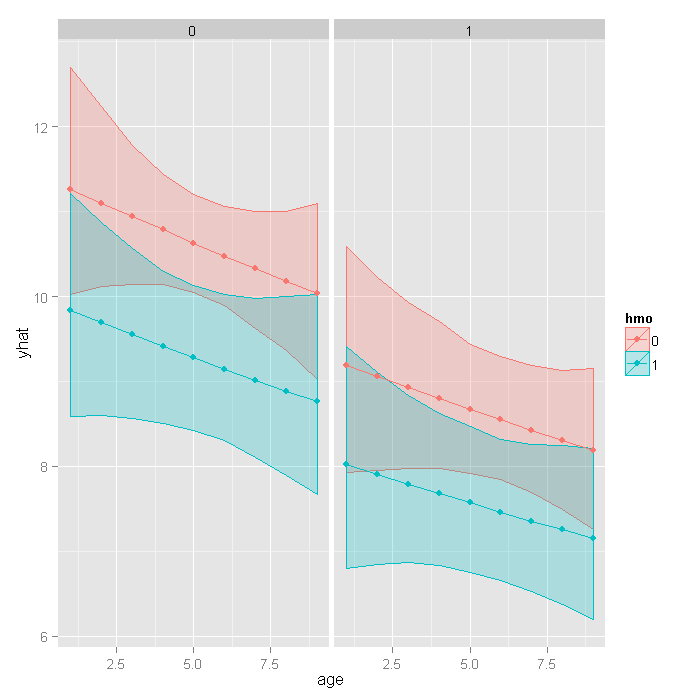
\includegraphics[width=0.8\linewidth]{hospitalstay2}
		
	\end{figure}
\end{frame}
\end{document}
